\subsection{Peak-to-Average Ratio}\label{subsec:peakratio}

In addition to examining traffic demands across the entire four-hour
prime-time window, we also explored how subscribers in the treatment
group exhibited different behavior for the 15-minute interval of highest (95th percentile)
demand in a day, regardless of prime-time hours. We measure the disparity
between a subscriber's daily 95th percentile and 
the mean usage as the \emph{peak-to-average ratio}
(PAR). This standard metric
shows the ratio of peak values to the effective value and extends those used
in conventional studies of user traffic patterns, such as the Sandvine's
peak traffic analysis~\cite{sandvine20141h}. 

\begin{figure}[t]
\centering
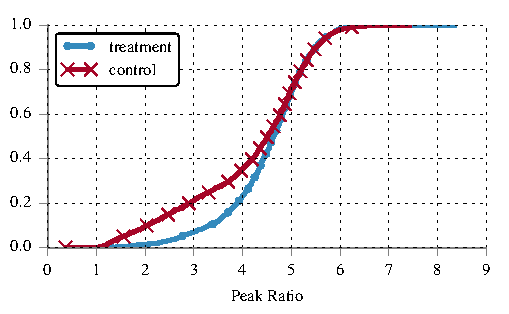
\includegraphics[width=.60\linewidth]{figures/peakratio_cdf_mean-devices.pdf}
\caption{Distribution of the daily peak-to-average ratio per subscriber, averaged for each subscriber over the measurement period in the treatment and  control groups.}
\label{fig:CDF-peak-ratio-mean}
\end{figure}

Figure~\ref{fig:CDF-peak-ratio-mean} shows the PAR for each 
subscriber in the treatment and control groups. The median PAR
 for subscribers from the treatment group is 4.64, compared to 4.51
for the control group.
We found that 40\% of the subscribers in both groups have PAR
greater than five; the PAR of subscribers in the treatment group is higher than those in the
control group, perhaps indicating that users in both higher service tiers do
in fact use the additional capacity for short periods of time. The
notable difference occurs for peak-to-average ratios of less-than 5: as
we observed in Section~\ref{subsec:behavior}, subscribers with more
moderate (median) traffic demands tend to increase their peak demand more in
response to the increased service tier.  Again, we believe these trends
appear not because users are necessarily eager to fill the additional
capacity of a higher service tier, but rather may be occurring because the upgrade
results in better performance, and that this improved user experience in
turn causes these subscribers to make more use of the Internet.

The lower prime-time ratio by volume, and a consistently higher
peak-to-average ratio per subscriber indicates the following:
subscribers in the treatment group have higher peak-to-average ratio than
those in the control group. However, these subscribers tend to still have
low absolute demand, so the relatively higher PAR for the treatment group does not significantly affect total traffic during prime-time and, when it is high, the demand
tends to be in non-prime-time hours.  Consistent with the results in
Section~\ref{subsec:primetime}, we also found that on weekdays, the
peak-to-average ratios in the treatment group are higher than the control
group, whereas on weekends peak-to-average ratios for both the control and
treatment groups are similar. 
